\documentclass[11pt]{scrartcl}
\usepackage[utf8]{inputenc}
\usepackage[sexy]{evanchen} 
\usepackage{graphicx}
\graphicspath{{8 Outsource K Math/Gambar/}}

\title{Projective Geometry}
\author{Azzam and Akeyla}

\begin{document}

\maketitle

\section{Cross-Ratio}
Diberikan empat titik segaris $A, B, X, Y$. Notasikan $(A, B; X, Y)$ sebagai cross-ratio yang didefinisikan sebagai \[(A, B; X, Y) = \dfrac{XA}{XB} \div \dfrac{YA}{YB}\]\\
Panjang garis-garis ini dapat bernilai negatif, sesuai dengan posisi titik-titiknya. Akibatnya, cross-ratio dapat bernilai negatif. Secara khusus, dapat dicek bahwa cross ratio ini bernilai positif jika dan hanya jika segmen garis $AB$ dan $XY$ tidak berpotongan atau ada segmen garis yang termuat di segmen garis yang lain (misal, urutannya $BXYA$ atau $XABY$).\\
$P(A, B; X, Y)$ disebut sebagai pensil dan merupakan himpunan empat garis $PA, PB, PX,$ dan $PY$ (lihat gambar \ref{fig:pencil}).\\

\begin{figure}[h!]
    \centering
    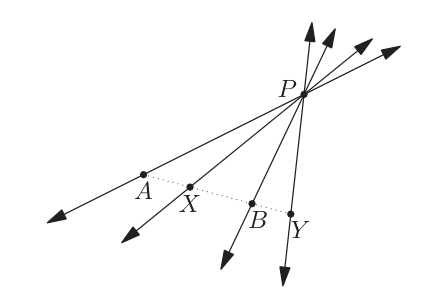
\includegraphics[width=0.5\linewidth]{pencil.png}
    \caption{Pensil $P(A, B; X, Y)$ (Sumber: EGMO - Evan Chen)}
    \label{fig:pencil}
\end{figure}
Cross-ratio juga dapat didefinisikan pada empat titik yang konsiklik, yakni untuk empat titik $A, B, X, Y$ yang konsiklik, definisikan \[(A, B; X, Y) = \dfrac{XA}{XB} \div \dfrac{YA}{YB}\]\\
Nilai cross-ratio ini positif saat segmen garis $AB$ dan $XY$ tidak berpotongan dan negatif pada kasus lainnya.\\
Nilai cross-ratio ini akan tetap sama apabila dilakukan proyeksi. Lihat gambar \ref{fig:line-proj}. Pensil $P(A, B; X, Y)$ diproyeksikan menjadi pensil $P(A', B'; X', Y')$. Pada kasus ini, kita akan punya $(A, B; X, Y) = (A', B'; X', Y')$. Kesamaan ini dapat dinotasikan sebagai $(A, B; X, Y) \stackrel{P}{=} (A', B'; X', Y')$ dan disebut sebagai "ambil perspektif terhadap $P$".

\begin{figure}[h!]
    \centering
    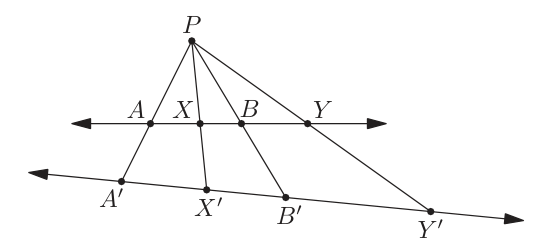
\includegraphics[width=0.5\linewidth]{proyeksigaris.png}
    \caption{Proyeksi titik $A, X, B, Y$ ke $A', X', B', Y'$ (Sumber: EGMO - Evan Chen)}
    \label{fig:line-proj}
\end{figure}

Demikian pula, kita akan memiliki nilai cross-ratio yang sama saat memproyeksikan empat titik yang konsiklik ke empat titik yang kolinear atau sebaliknya. Perhatikan gambar \ref{fig:cline-proj}. Berlaku juga $(A, B; X, Y) \stackrel{P}{=} (A', B'; X', Y')$
\begin{figure}[h!]
    \centering
    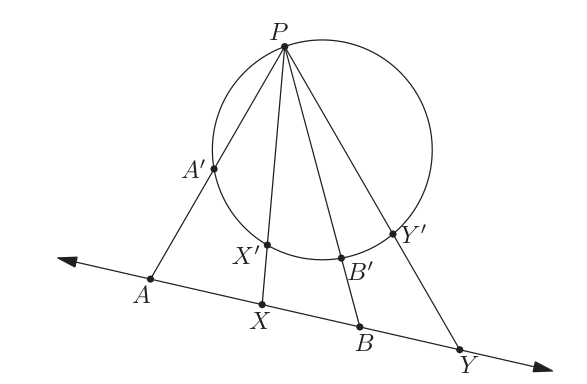
\includegraphics[width=0.5\linewidth]{cline-proj.png}
    \caption{Proyeksi titik $A, X, B, Y$ ke $A', X', B', Y'$ (Sumber: EGMO - Evan Chen)}
    \label{fig:cline-proj}
\end{figure}

\section{Harmonic Bundle}
Saat $(A, B; X, Y) = -1$, kita menyebut $(A, B; X, Y)$ sebagai harmonic bundle (atau lebih seringnya, hanya harmonic). Apabila segiempat siklik $AXBY$ memenuhi $(A, B; X, Y) = -1$, maka $AXBY$ disebut sebagai segiempat harmonik.\\
Untuk seterusnya, kita akan menemui istilah "titik di tak hingga" (en: point at infinity) yang biasa dilambangkan dengan $P_{\infty}$. Dua garis yang sejajar akan berpotongan pada titik ini. Untuk memahami titik ini, bayangkan diri anda berada di sebuah jalan yang lurus dan anda melihat ke arah jalan tersebut. Kedua sisi jalan yang sejajar akan terlihat akan menyempit dan terlihat akan berpotongan. Titik inilah yang disebut sebagai titik di tak hingga bagi kedua garis tersebut.\\
Beberapa properti dan lemma yang berguna:
\begin{enumerate}
    \item \label{properti1} Diberikan titik $A$ dan $B$. Titik $M$ adalah titik tengah $AB$. Titik $P_{\infty}$ adalah titik di tak hingga pada garis $AB$. Maka, $(A, B; M, P_{\infty})$ harmonic
    \item \label{properti2}  Diberikan sebuah lingkaran $\omega$ dan titik $P$ yang ada di luar lingkaran. Misalkan $PX$ dan $PY$ adalah garis singgung $\omega$ dan $X, Y$ terletak di $\omega$. Titik $A$ dan $B$ terletak di lingkaran $\omega$ sedemikian hingga $P, A, B$ segaris. Maka, $AXBY$ adalah segiempat harmonic dan jika $Q$ adalah perpotongan $AB$ dan $XY$ maka $(A, B; Q, P)$ harmonic. 
    \item \label{properti3} Diberikan segitiga $ABC$ dengan titik $D, E, F$ secara berturut-turut terletak di $BC, CA, AB$ dan $AD, BE, CF$ berpotongan di satu titik. Misal $X$ adalah titik perpotongan $EF$ dan $BC$. Maka, $(X, D; B, C)$ harmonic
    \item \label{properti4} Diberikan titik $X, A, Y, B$ yang segaris dengan urutan tersebut. Titik $C$ tidak segaris dengan keempat titik sebelumnya. Maka, dua dari tiga kondisi yang diberikan akan mengakibatkan kondisi lainnya terpenuhi:
    \begin{enumerate}
        \item $(A, B; X, Y)$ harmonic
        \item $\angle{XCY} = 90^{\circ}$
        \item $CY$ membagi sudut $\angle{ACB}$ sama besar
    \end{enumerate}
 \end{enumerate}

\section{Contoh Soal}
\begin{example}
    $AD$ adalah garis tinggi dari segitiga $ABC$. Titik $P$ terletak di segmen garis $AD$. Garis $BP$ dan $AC$ berpotongan di $E$. Garis $CP$ dan $AB$ berpotongan di $F$. Buktikan bahwa garis $AD$ adalah garis bagi sudut $\angle{EDF}$.
\end{example}

\begin{proof}[Solusi:]
    Misalkan $X$ adalah perpotongan $EF$ dan $BC$ dan $Y$ adalah perpotongan $AD$ dan $EF$. Dengan properti \ref{properti3}, didapat $(B, C; D, X)$ harmonic. Kemudian, dengan memproyeksikan pensil $A(B, C; D, X)$ ke $EF$, didapat $(F, E; Y, X)$ juga harmonic. Terakhir, dengan menggunakan properti $\ref{properti4}$ pada pensil $D(X, Y; F, E)$, didapat $YD$ merupakan garis bagi sudut $\angle{FDE}$, yakni $AD$ adalah garis bagi sudut $\angle{FDE}$
\end{proof}

\section{Soal}
\begin{problem}
    $A, C, B, D$ terletak pada satu garis dengan urutan tersebut dan $(A, B; C, D)$ harmonic. Titik $M$ adalah titik tengah $AB$. Buktikan bahwa $AM^2 = MC \cdot MD$ dan $DC\cdot DM = DB\cdot DA$
\end{problem}

\begin{problem}
    Beberapa properti segiempat harmonic. Diberikan segiempat siklik $ABCD$ harmonic dengan urutan tersebut yang ada di lingkaran $\omega$. Misalkan $M$ adalah titik tengah $AC$. Buktikan:
    \begin{enumerate}
        \item Garis singgung $\omega$ pada titik $A$ dan $C$ serta garis $BD$ akan konkuren atau ketiganya sejajar (secara teknis, kita bisa bilang semuanya konkuren karena ketiganya sejajar = konkuren di titik di tak hingga)
        \item $BD$ adalah symmedian dari titik $B$ di segitiga $ABC$ dan symmedian dari titik $D$ di segitiga $ADC$ (tergantung definisi, ini bisa jadi trivial)
        \item Sudut $\angle{BMC}$ sama dengan $\angle{DMC}$
        \item Garis bagi sudut $\angle{ABC}$ dan $\angle{ADC}$ berpotongan di sisi $AC$
    \end{enumerate}
\end{problem}

\begin{problem}
    Pada segitiga $ABC$ dengan titik tinggi $H$, konstruksi garis singgung dari $A$ ke lingkaran dengan diameter $BC$. Asumsikan kedua garis singgung menyinggung lingkaran dengan diameter $BC$ di $P$ dan $Q$. Buktikan bahwa $P, H, Q$ segaris.
\end{problem}

\begin{problem}
    Misalkan $ABC$ adalah segitiga lancip. Lingkaran $\omega$ adalah lingkaran yang berpusat di $O$ dan melalui titik $B$ dan $C$ serta memotong sisi $AB$ dan $AC$ di $E$ dan $F$. Lingkaran luar $AEF$ memotong lingkaran luar $ABC$ di titik $M$. Buktikan bahwa $\angle{OMA} = 90^{\circ}$.
\end{problem}

\begin{problem}
    Segiempat $ABCD$ memiliki lingkaran luar $\omega$ dengan pusat $O$. $AC \cap BD \equiv P$. Lingkaran luar $ABP$ dan $CDP$ berpotongan di $P$ dan $Q$. Asumsikan titik $O, P, Q$ berbeda semua. Buktikan $\angle{OQP} = 90^{\circ}$.
\end{problem}

\begin{problem}
    (USAJMO 2011) Titik $A, B, C, D, E$ terletak di lingkaran $\omega$ dan titik $P$ terletak di luar lingkaran $\omega$ sedemikian hingga:
    \begin{enumerate}
        \item Garis $PB$ dan $PD$ adalah garis singgung $\omega$
        \item $P, A,$ dan $C$ segaris
        \item $DE$ sejajar dengan $AC$
    \end{enumerate}
    Buktikan bahwa $BE$ membagi $AC$ sama panjang.
    % https://artofproblemsolving.com/community/c5h404355p2254813
\end{problem}

\begin{problem}
    (Norwegia MO 2022) Diberikan sebuah segitiga $ABC$ dengan lingkaran luar $\omega$ dan $AB > AC$. Titik $X$ dan $Y$ yang berbeda dari $A$ terletak di keliling $\omega$ sedemikian hingga $AX$ melewati titik tengah $BC$ dan $AY$ melewati proyeksi titik $A$ ke $BC$. Diketahui bahwa $XY$ sejajar dengan $BC$. Tentukan besar sudut $\angle CAB$.
    % https://artofproblemsolving.com/community/c6t45819f6h3275823_in_triangle_with_ab_gt_ac_find_angle_bac
\end{problem}

\begin{problem}
    (KTOM Mei 2020) Diberikan segitiga $ABC$ dengan median (garis berat) dari titik $A$ memotong lingkaran luar $ABC$ di titik $D$. Di dalam segitiga $ABC$, terdapat titik $P$ pada median $A$. Diketahui $BP$ dan $CP$ memotong $AC$ dan $AB$ berturut-turut di titik $E$ dan $F$. Selanjutnya, diketahui $DE$ dan $DF$ memotong lingkaran luar $ABC$ lagi di titik $X$ dan $Y$. Buktikan bahwa untuk setiap titik $P$ yang ada, garis $XY$ akan konkuren di suatu titik.
\end{problem}

\end{document}